\chapter{PTAGPU} \label{chap:main}
This thesis presents a software library named PTAGPU, the name is derived from pointer analysis (PTA) and graphics processing unit (GPU).
As the name suggests the core idea is to use GPUs for the purpose of performing a pointer analysis.
The library PTAGPU was developed as a whole program analysis module inside the SVF framework which is in turn built on top of the LLVM compiler system.
\section{Integrating PTAGPU into SVF}
As described in \autoref{sec:svf} the SVF framework is capable of processing the LLVM-IR of a compiled program and capture the individual LLVM-IR instructions in a program assignment graph.
When SVF is launched for a whole program analysis, the program assignment graph is further processed into a constraint graph that holds holds all relevant constraints for an initial pointer analysis, see \autoref{tab:ander}.
At this point the constraint graph is passed into a class that inherits from the PointerAnalysis class, see \autoref{fig:pta-svf} for an overview of the pointer analysis class hierarchy in SVF.
Since our goal is to implement a custom pointer analysis, we can inject out own implementation at this stage as a PointerAnalysis subclass.
Specifically we inherit from the Andersen class which is itself a subclass of the PointerAnalysis class that implements the Andersen inclusion-based pointer analysis algorithm in SVF.
By extensive use of runtime polymorphism most of SVF is implemented via virtual member functions - a construct specific to c++ - allowing for function overriding in subclasses. This makes implementing a custom pointer analysis easy as we can reuse most of the initialization steps and program assignment graph processing from the superclasses. Part of the processing is an initial topological sorting and the previously mentioned interpretation into a constraint graph.
As a result we end up with a constraint graph and all strongly connected components of said graph when we initialize our PTAGPU class that inherits from the Andersen class.
The in-memory representation of constraint graphs or generic graphs in SVF is more akin to a linked list data structure where each node carries references to all outgoing and incoming edges and those edges carry references to source and destination nodes as well as auxiliary information, which is an ideal memory model for iterative algorithms such as the default Andersen algorithm where the algorithm works from one node to the next.
Unfortunately this memory model is not ideal for parallel processing.
For this reason we initially reinterpret the constraint graph into a more fitting data structure.
While iterating through the entire constraint graph, we differentiate by edge types and collect all $(src,dst)$ edge pairs in standard library vectors.
If we refer back to the design principles of SVF in \autoref{sec:svf}, where pointer analyses were conceptually split into three components, the Rules, the Graph and the Solver, we effectively implement our own Graph component by using a different linear memory representation for the constraint graph. 
The underlying goal of putting the constraint graph into a linear in-memory data structure is to allow us to more easily copy the memory region containing the relevant information into GPU device memory, which is where our pointer analysis will operate on the data.
Similarly to the Graph component we also modify the Solver and Rule components in the custom analysis implementation.
The details of the implementation will be described in detail in \autoref{sec:design}.

\section{Goal of the Algorithm}
Our goal is to use the provided program assigment graph from SVF and the derived constraint graph to compute a points-to set for each pointer variable in the program.
Overall our algorithm is supposed to serve as an initial pointer analysis pass in the SVF framework. Together with the pointer information we can then proceed to build an over approximated call graph.
One might assume that no pointer information is needed for SVF to build a call graph for the program. Unfortunately indirect function invocations, where function are accessed by pointer dereferencing itself, requires us to build pointer information in order to create an over approximated sound call graph. The over approximate nature stems from the imprecision of Andersen's analysis. This limitation always remains, no matter the algorithm, since pointer analyses are fundamentally undecidable as was mentioned in \autoref{sec:pta}.
It is important to consider that the initial pointer analysis does not directly produce any valuable information in terms of static analysis purposes. Instead we use the pointer information produced by the initial analysis for the call graph which is then used to refine the analysis result by applying a more precise flow- and/or context-sensitive analysis that produces the relevant results, which can then be used to derive value flow information that can directly be used for actual analysis purposes.
Since we are applying a more precise pointer analysis at a later stage anyways one might argue that it would be wise to start off with such an analysis. For small programs this is a viable strategy, unfortunately these more precise analyses are currently not scalable for a whole program analysis and are only applied on-demand \cite{sui2016svf}. This is also one of the motivations for trying to accelerate the initial Anderen analysis specifically since it is performed on the entire program and thus can in theory profit from the paralellism of GPUs.

\section{Design of the Algorithm}\label{sec:design}
The PTAGPU library uses CUDA\footnote{\url{https://developer.nvidia.com/cuda-toolkit}}, an application programming interface language from NVIDIA, to program GPUs in C++.
CUDA accomodates developers with a collection of abstractions that simplify operations with GPU compute and memory. NVIDIA also provides a standalone library for common parallel oeprations such as sorting and transformations named Thrust\footnote{\url{https://docs.nvidia.com/cuda/thrust/index.html}} which is also employed by PTAGPU for common sorting and deduplication operations.
In principle all calculations that are executed with a GPU are denoted as kernels in CUDA. While GPU kernels and CPU code can be shared, CUDA provides some intrinsic operations that can only function when executed on a GPU.
Likewise all CPU operations that rely on external libraries or non standard-library code are not supported in GPU kernels.

\subsection{CUDA Architecture}
The CUDA programming model revolves around blocks of threads. Each block of a kernel executes the same code with the same number of threads.
Thread blocks are further divided into Warps, which are a collection of 32 threads each. This type of parallel processing is called SIMT, for single instruction, multiple threads.
In reality a Warp is more analogous to a single vectorized operation that executes 32 units of work or lanes at once than a collection of individual threads, although each thread in a Warp has its own instruction address counter. Having instruction address counters per thread allows independent branching, resulting in thread divergence. The divergence is implemented by executing each conditional branch sequentially for all threads in a Warp and disabling the threads that do not execute the specific branch.
This way each thread in a Warp always executes the same instruction if active. Since branches are not executed in parallel, thread divergence is discouraged if possible for performance reasons.
These specifications of Warps are uniform in all CUDA hardware and resemble a single group of work that can be scheduled on the device specific number of multiprocessors.
To more easily differentiate between different generations of hardware, the CUDA programming model is segmented into tiers of compute capabilities, where newer hardware with newer capabilities receives a higher compute capability.
Each CUDA capable device has a number of streaming multiprocessors, in short SMs, which themselves have a certain amount of L1 shared memory and number of registers per core among other resources. 
While this is similar to how CPU cores operate, GPU programming uses a flat memory hierarchy with less reliance on caching and more on raw memory bandwidth. For this reason each core in an SM has a relatively large register file so that a single CUDA thread commonly uses hundreds of registers.
The entire work that is to be performed by a single kernel is called a grid, which is divided evenly into blocks, which are divided into Warps. Both the grid and each block can be indexed in up to three dimensions, which is useful for working with shader, global illumination rendering and less useful for static analyses.
To start a computation, a collection of thread blocks are assigned to the available SMs of a GPU. Depending on the hardware and compute capability, a single SM can execute multiple Warps from the assigned thread blocks in parallel as long as enough resources are available in the SM.
\begin{figure}
    \centering
    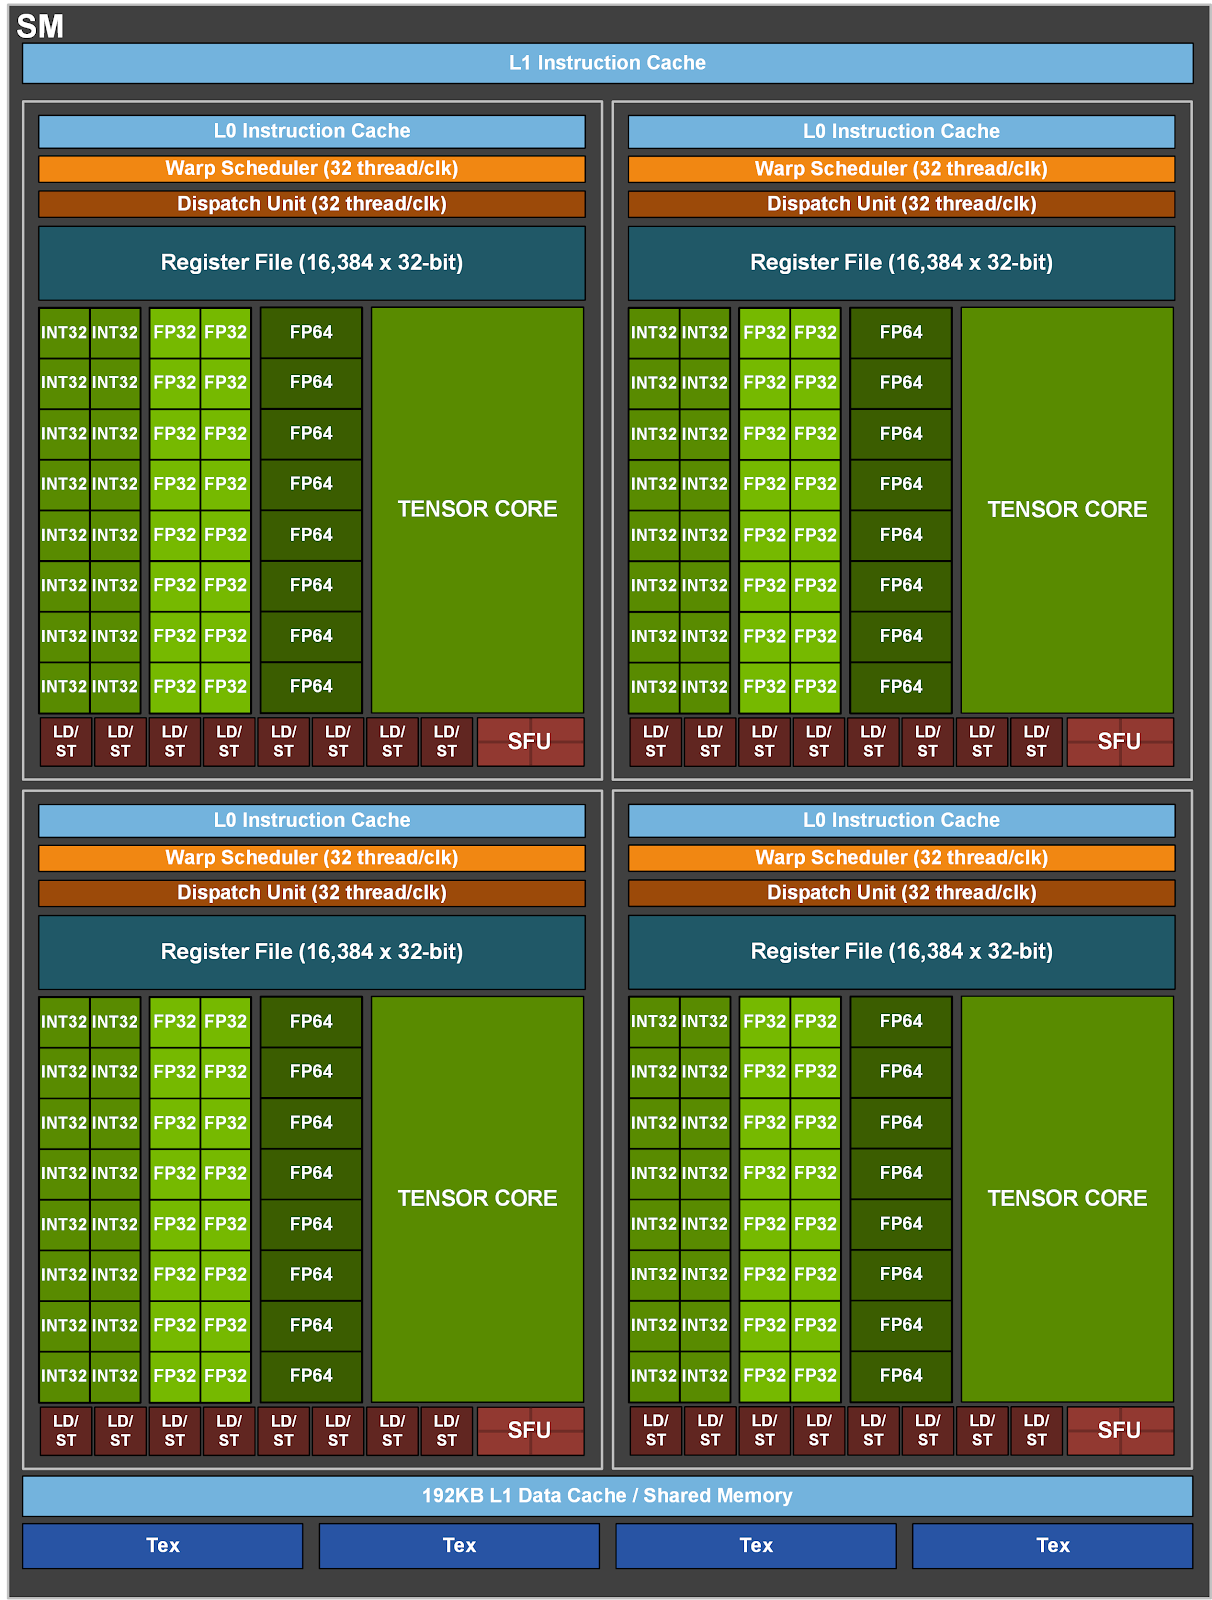
\includegraphics[width=.7\textwidth]{img/a100.png}
    \caption[Diagram of a single A100 SM]{A single SM of an A100 GPU.\\Taken from an NVIDIA Blog Post\footnotemark}
    \label{fig:cuda-sm}
\end{figure}
\footnotetext{\url{https://developer.nvidia.com/blog/nvidia-ampere-architecture-in-depth/}}
The execution order of individual Warps is handled by a Warp scheduler, that decides what Warps get executed at what time.
The purpose of overprovisioning SMs with more blocks/Warps than they can concurrently execute is that when a single Warp executes a memory read/write operation other Warps can execute while the device is busy fetching the data.
Key specification for each SM of a certain compute capability are the following:
\begin{itemize}
    \item Memory Bandwith per SM
    \item Total shared memory per SM
    \item Max number of threads per SM
    \item Max number of blocks per SM
    \item Total number of registers of all cores in SM
\end{itemize}

\subsubsection{Occupancy}
Since each SM has multiple limited resources that can be controlled by the developer, namely register count, shared memory and thread count, a kernel has to be designed with these limitations in mind such that a maximally concurrent execution is possible.
Given a device with compute capability 8.0 and a kernel that requires 256 registers per thread while also running 256 threads per block, we would essentially limit our execution to a single block per SM, since a device with compute capability 8.0 has 64K registers per SM.
This might be disadvantageous, since the SM is in theory capable of working on up to 1024 threads.
We might profit from reducing the amount of registers used per thread and thus increasing the occupancy on our GPU.
Counterintuitively high occupancy does not always lead to better performance. Some programs disproportionally profit from the use of a single resource.
For example compute intensive kernels require more registers per thread than kernels that are heavily reliant on memory operations. Increasing the use of shared memory does not always lead to a performance improvement and decreasing the number of required registers is not always possible.
\subsubsection{Memory Accesses in CUDA}
While modern GPUs can in theory perform multiple TFLOPS of calculations per second, effectively all calculations are limited by memory bandwidth.
Consequently, how we access the GPU memory is very important for the overall performance of our analysis. Specifically coalesced memory accesses of individual Warps where consecutive threads access consecutive memory addresses are important so the memory read operation can be performed within a single transaction and not multiple strided reads.
\begin{figure}
    \centering
    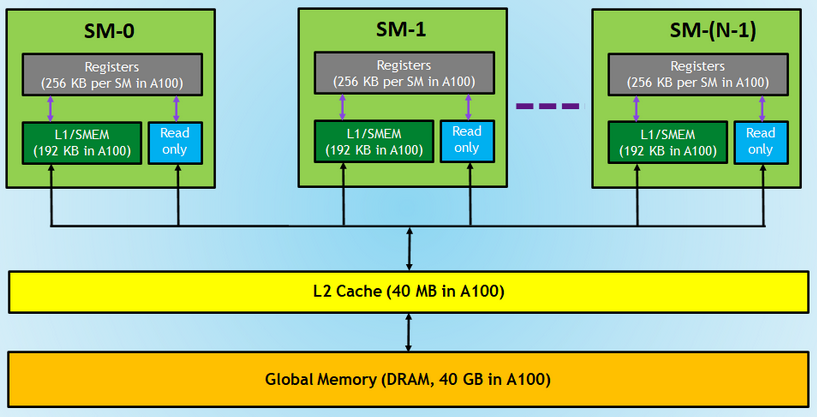
\includegraphics[width=.7\textwidth]{img/cuda.png}
    \caption{Diagram of the CUDA memory architecture for an A100 GPU.\\Taken from \cite{cudarefresher}.}
    \label{fig:cuda-arch}
\end{figure}
The GPU memory controller on modern graphics cards can typically execute memory read or write operations in granularities of 32 bytes up to 128 bytes in total.
As a result it is for example more efficient to load a single byte of memory per thread in a Warp, compared to loading 8 bytes per thread, since we would exceed the maximum of 128 bytes per memory transaction and require multiple memory accesses.
In terms of time needed per instruction, global memory operations are typically two orders of magnitude slower compared to operations on SM registers or shared memory in L1 cache. For this reason CUDA programs can perform exponentially worse if memory accesses are random or strided inefficiently instead of coalesced.

\subsubsection{Unified Memory}
When CUDA code is executed on a 64-bit host system, the developer can use a single memory address space for host and device memory.
Using this unified memory address space allows memory access from both CPU and GPU in the same address space without explicit memory copy operations.
The memory in question is moved implicitly to the device that performs the read operation. The CUDA API also allows the developer to assign preferred residency for specific memory regions, as well as prefetching memory asynchronously for a device. When prefetching is properly employed, unified memory achieves the same performance as dedicated device memory \cite{cudaunifiedmem}.
The major advantage of unified memory is the fact that the memory allocation size is only limited by system memory, not device memory.
This allows a CUDA program to potentially hold vastly more data in memory than would be possible with only GPU memory, while also moving the needed memory regions without much involvement of the developer.
Crucially this keeps large data structures intact without splitting and partitioning them for incremental loading into GPU memory.
This mirrors some of the core ideas of Graspan \autoref{sec:graspan} where parts of the graph are written to disk to conserve memory usage.
Since many high performance computing environments have vastly more main memory available than individual GPUs have device memory, this enables us to expand the scope of our analysis without requiring specialized GPU hardware.

\subsection{Initialization of CUDA code}
As soon as the constraint graph is handed over to the CUDA section of the code some global state is initialized with the information from the constraint graph.
This includes various counter variables for the number of nodes in the graph, as well as the initial unified memory allocations.
When the counter for the number of nodes is first initialized the node count is read from the constraint graph and increased by 20 percent to reserve headroom for new nodes that might be added to the constraint graph during the execution of the algorithm.
This ensures that each node has a well defined place in memory that can not be overwritten by subsequent nodes.
In the current implementation, the algorithm allocates a fixed amount of unified memory accessible from the CPU and GPU. While this requires overprovisioning of memory for a given analysis without knowing the exact amount needed for the pointer analysis, dynamic allocation proves to be very challenging as it is difficult to deduce the exact required amount of GPU memory from a given constraint graph for pointer analysis.


based on \cite{mendez2010parallel} and \cite{mendez2012gpu}

\begin{center}
    \begin{bytefield}{32}
        \begin{rightwordgroup}{includes all pointer relations\\that have been computed\\at any stage}
            \memsection{ffff ffff}{a000 0000}{12}{pointer constraints}
        \end{rightwordgroup}\\
        \begin{rightwordgroup}{these memory regions are used\\to compute the delta updates\\for the pointer relations}
            \memsection{9fff ffff}{6000 0000}{8}{current pointer constraints}\\
            \memsection{5fff ffff}{2000 0000}{8}{next pointer constraints}
        \end{rightwordgroup}\\
        \begin{rightwordgroup}{static memory\\does not change once written}
            \memsection{1fff ffff}{1000 0000}{2}{load constraints}\\
            \memsection{0fff ffff}{0000 0000}{2}{store constraints}
        \end{rightwordgroup}\\
    \end{bytefield}
\end{center}

\begin{center}
    \begin{bytefield}{32}
        \bitheader{0-31} \\
        \bitbox{4}{Four} & \bitbox{8}{Eight} &
        \bitbox{16}{Sixteen} & \bitbox{4}{Four}
    \end{bytefield}
\end{center}
\blindtext[1]
\begin{center}
    \definecolor{lightcyan}{rgb}{0.84,1,1}
    \definecolor{lightgreen}{rgb}{0.64,1,0.71}
    \definecolor{lightred}{rgb}{1,0.7,0.71}
    \begin{bytefield}[bitheight=\widthof{~Base~},
            boxformatting={\centering\small},rightcurly=., rightcurlyspace=0pt]{32}
        % \bitlabel{29}{Data} & \bitlabel{1}{Base} & \bitlabel{2}{Next} \\
        \bitheader{0,28,29,30,31} \\
        \begin{rightwordgroup}{
                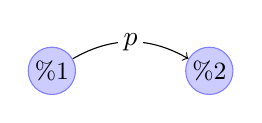
\begin{tikzpicture}
                    \tikzstyle{node}=[circle, draw=blue!50, fill=blue!20, inner sep=1pt, minimum size=6mm]
                    \tikzstyle{linenode}=[pos=0.5,fill=white,inner sep=2pt,outer sep=2pt]
                    \node[node] (A) at (0,0) {\small$\%1$};
                    \node[node] (B) at (2,0) {\small$\%2$};
                    \path [->] (A) edge[bend left] node[linenode] {$p$} (B);
                \end{tikzpicture}
            }
            \bitbox{29}[bgcolor=lightred]{Data} &
            \bitbox{1}[bgcolor=lightcyan]{\rotatebox{90}{Base}} &
            \bitbox{2}[bgcolor=lightgreen]{\rotatebox{90}{Next}}
        \end{rightwordgroup}
    \end{bytefield}
\end{center}
\begin{center}
    \definecolor{lightcyan}{rgb}{0.84,1,1}
    \definecolor{lightgreen}{rgb}{0.64,1,0.71}
    \definecolor{lightred}{rgb}{1,0.7,0.71}
    \begin{bytefield}[bitheight=\widthof{~Base~},
            boxformatting={\centering\small},rightcurly=., rightcurlyspace=0pt, bitwidth=11pt]{32}
        \bitheader{0-31} \\
        \begin{rightwordgroup}{Words}
            \bitbox{29}[bgcolor=lightred]{Data} &
            \bitbox{1}[bgcolor=lightcyan]{\rotatebox{90}{Base}} &
            \bitbox{2}[bgcolor=lightgreen]{\rotatebox{90}{Next}}
        \end{rightwordgroup}
    \end{bytefield}
\end{center}
\blindtext[1]

\subsection{Sparse Bitvectors}
\subsection{Memory Layout}
\subsubsection{Unified Memory}
\subsubsection{64bit Addresses}
\subsection{Concurrent Graph Rewriting}
\subsection{Integration with SVF}
\subsubsection{Parallelizing SVF}
\section{Experimental Results}
\subsection{Test Suite}
\subsection{Bemchmark Suite}
\section{Evaluation}
